\documentclass[10pt]{article}
\usepackage[T1]{fontenc}

% Document Details
\newcommand{\CLASS}{AMATH 515}
\newcommand{\assigmentnum}{Problem Set 1}

\usepackage[margin = 1.5in]{geometry}
\usepackage{titling}
\setlength{\droptitle}{-6em}   % This is your set screw
\date{}
\renewcommand{\maketitle}{
	\clearpage
	\begingroup  
	\centering
	\LARGE \sffamily\textbf{\CLASS} \Large \assigmentnum\\[.8em]
	\large Tyler Chen\\[1em]
	\endgroup
	\thispagestyle{empty}
}
 % Title Styling


\usepackage{enumitem}

% Figures
\usepackage{subcaption}

% TikZ and Graphics
\usepackage{tikz, pgfplots}
\pgfplotsset{compat=1.12}
\usetikzlibrary{patterns,arrows}
\usepgfplotslibrary{fillbetween}

\usepackage{pdfpages}
\usepackage{adjustbox}

\usepackage{lscape}
\usepackage{titling}
\usepackage[]{hyperref}


% Header Styling
\usepackage{fancyhdr}
\pagestyle{fancy}
\lhead{\sffamily \CLASS}
\rhead{\sffamily Chen \textbf{\thepage}}
\cfoot{}

% Paragraph Styling
\setlength{\columnsep}{1cm}
\setlength{\parindent}{0pt}
\setlength{\parskip}{5pt}
\renewcommand{\baselinestretch}{1}

% TOC Styling
\usepackage{tocloft}
\iffalse
\renewcommand{\cftsecleader}{\cftdotfill{\cftdotsep}}

\renewcommand\cftchapafterpnum{\vskip6pt}
\renewcommand\cftsecafterpnum{\vskip10pt}
\renewcommand\cftsubsecafterpnum{\vskip6pt}

% Adjust sectional unit title fonts in ToC
\renewcommand{\cftchapfont}{\sffamily}
\renewcommand{\cftsecfont}{\bfseries\sffamily}
\renewcommand{\cftsecnumwidth}{2em}
\renewcommand{\cftsubsecfont}{\sffamily}
\renewcommand{\cfttoctitlefont}{\hfill\bfseries\sffamily\MakeUppercase}
\renewcommand{\cftaftertoctitle}{\hfill}

\renewcommand{\cftchappagefont}{\sffamily}
\renewcommand{\cftsecpagefont}{\bfseries\sffamily}
\renewcommand{\cftsubsecpagefont}{\sffamily}
\fi
 % General Styling
% Code Display Setup
\usepackage{listings,lstautogobble}
\usepackage{lipsum}
\usepackage{courier}
\usepackage{catchfilebetweentags}

\lstset{
	basicstyle=\small\ttfamily,
	breaklines=true, 
	frame = single,
	rangeprefix=,
	rangesuffix=,
	includerangemarker=false,
	autogobble = true
}


\usepackage{algorithmicx}
\usepackage{algpseudocode}

\newcommand{\To}{\textbf{to}~}
\newcommand{\DownTo}{\textbf{downto}~}
\renewcommand{\algorithmicdo}{\hspace{-.2em}\textbf{:}}
 % Code Display Setup
% AMS MATH Styling
\usepackage{amsmath, amssymb}
\newcommand{\qed}{\hfill\(\square\)}

%\newtheorem*{lemma}{Lemma} 
%\newtheorem*{theorem}{Theorem}
%\newtheorem*{definition}{Definition}
%\newtheorem*{prop}{Proposition}
%\renewenvironment{proof}{{\bfseries Proof.}}{}


% mathcal
\newcommand{\cA}{\ensuremath{\mathcal{A}}}
\newcommand{\cB}{\ensuremath{\mathcal{B}}}
\newcommand{\cC}{\ensuremath{\mathcal{C}}}
\newcommand{\cD}{\ensuremath{\mathcal{D}}}
\newcommand{\cE}{\ensuremath{\mathcal{E}}}
\newcommand{\cF}{\ensuremath{\mathcal{F}}}
\newcommand{\cG}{\ensuremath{\mathcal{G}}}
\newcommand{\cH}{\ensuremath{\mathcal{H}}}
\newcommand{\cI}{\ensuremath{\mathcal{I}}}
\newcommand{\cJ}{\ensuremath{\mathcal{J}}}
\newcommand{\cK}{\ensuremath{\mathcal{K}}}
\newcommand{\cL}{\ensuremath{\mathcal{L}}}
\newcommand{\cM}{\ensuremath{\mathcal{M}}}
\newcommand{\cN}{\ensuremath{\mathcal{N}}}
\newcommand{\cO}{\ensuremath{\mathcal{O}}}
\newcommand{\cP}{\ensuremath{\mathcal{P}}}
\newcommand{\cQ}{\ensuremath{\mathcal{Q}}}
\newcommand{\cR}{\ensuremath{\mathcal{R}}}
\newcommand{\cS}{\ensuremath{\mathcal{S}}}
\newcommand{\cT}{\ensuremath{\mathcal{T}}}
\newcommand{\cU}{\ensuremath{\mathcal{U}}}
\newcommand{\cV}{\ensuremath{\mathcal{V}}}
\newcommand{\cW}{\ensuremath{\mathcal{W}}}
\newcommand{\cX}{\ensuremath{\mathcal{X}}}
\newcommand{\cY}{\ensuremath{\mathcal{Y}}}
\newcommand{\cZ}{\ensuremath{\mathcal{Z}}}

% mathbb
\usepackage{bbm}
\newcommand{\bOne}{\ensuremath{\mathbbm{1}}}

\newcommand{\bA}{\ensuremath{\mathbb{A}}}
\newcommand{\bB}{\ensuremath{\mathbb{B}}}
\newcommand{\bC}{\ensuremath{\mathbb{C}}}
\newcommand{\bD}{\ensuremath{\mathbb{D}}}
\newcommand{\bE}{\ensuremath{\mathbb{E}}}
\newcommand{\bF}{\ensuremath{\mathbb{F}}}
\newcommand{\bG}{\ensuremath{\mathbb{G}}}
\newcommand{\bH}{\ensuremath{\mathbb{H}}}
\newcommand{\bI}{\ensuremath{\mathbb{I}}}
\newcommand{\bJ}{\ensuremath{\mathbb{J}}}
\newcommand{\bK}{\ensuremath{\mathbb{K}}}
\newcommand{\bL}{\ensuremath{\mathbb{L}}}
\newcommand{\bM}{\ensuremath{\mathbb{M}}}
\newcommand{\bN}{\ensuremath{\mathbb{N}}}
\newcommand{\bO}{\ensuremath{\mathbb{O}}}
\newcommand{\bP}{\ensuremath{\mathbb{P}}}
\newcommand{\bQ}{\ensuremath{\mathbb{Q}}}
\newcommand{\bR}{\ensuremath{\mathbb{R}}}
\newcommand{\bS}{\ensuremath{\mathbb{S}}}
\newcommand{\bT}{\ensuremath{\mathbb{T}}}
\newcommand{\bU}{\ensuremath{\mathbb{U}}}
\newcommand{\bV}{\ensuremath{\mathbb{V}}}
\newcommand{\bW}{\ensuremath{\mathbb{W}}}
\newcommand{\bX}{\ensuremath{\mathbb{X}}}
\newcommand{\bY}{\ensuremath{\mathbb{Y}}}
\newcommand{\bZ}{\ensuremath{\mathbb{Z}}}

% alternative mathbb
\newcommand{\NN}{\ensuremath{\mathbb{N}}}
\newcommand{\RR}{\ensuremath{\mathbb{R}}}
\newcommand{\CC}{\ensuremath{\mathbb{C}}}
\newcommand{\ZZ}{\ensuremath{\mathbb{Z}}}
\newcommand{\EE}{\ensuremath{\mathbb{E}}}
\newcommand{\PP}{\ensuremath{\mathbb{P}}}
\newcommand{\VV}{\ensuremath{\mathbb{V}}}
\newcommand{\cov}{\ensuremath{\text{Co}\VV}}
% Math Commands

\newcommand{\st}{~\big|~}
\newcommand{\stt}{\text{ st. }}
\newcommand{\ift}{\text{ if }}
\newcommand{\thent}{\text{ then }}
\newcommand{\owt}{\text{ otherwise }}

\newcommand{\norm}[1]{\left\lVert#1\right\rVert}
\newcommand{\snorm}[1]{\lVert#1\rVert}
\newcommand{\ip}[1]{\ensuremath{\left\langle #1 \right\rangle}}
\newcommand{\pp}[3][]{\frac{\partial^{#1}#2}{\partial #3^{#1}}}
\newcommand{\dd}[3][]{\frac{\d^{#1}#2}{\d #3^{#1}}}
\renewcommand{\d}{\ensuremath{\mathrm{d}}}

\newcommand{\indep}{\rotatebox[origin=c]{90}{$\models$}}




 % Math shortcuts
\usepackage{mdframed}

\newenvironment{algorithm}[1][\@nil]
{\def\tmp{#1}%
\begin{mdframed}[
  frametitle={Algorithm. \ifx\tmp\@nnil  \else \normalfont (#1) \fi},
  linecolor=green!70,
  linewidth=1,
  topline=false,
  bottomline=false,
  rightline=false,
  rightmargin=.5cm
]}
{\end{mdframed}}

\newenvironment{method}[1][\@nil]
{
\def\tmp{#1}%
\begin{mdframed}[
  frametitle={Method. \ifx\tmp\@nnil  \else \normalfont (#1) \fi},
  linecolor=violet!70,
  linewidth=1,
  topline=false,
  bottomline=false,
  rightline=false,
  rightmargin=.5cm
]}
{\end{mdframed}}

\newenvironment{definition}[1][\@nil]
{\def\tmp{#1}%
\begin{mdframed}[
  frametitle={Definition. \ifx\tmp\@nnil  \else \normalfont (#1) \fi},
  linecolor=blue!70,
  linewidth=1,
  topline=false,
  bottomline=false,
  rightline=false,
  rightmargin=.5cm
]}
{\end{mdframed}}

\newenvironment{theorem}[1][\@nil]
{\def\tmp{#1}%
\begin{mdframed}[
  frametitle={Theorem. \ifx\tmp\@nnil  \else \normalfont (#1) \fi},
  linecolor=red!70,
  linewidth=1,
  topline=false,
  bottomline=false,
  rightline=false,
  rightmargin=.5cm
]}
{\end{mdframed}}

\newenvironment{lemma}[1][\@nil]
{\def\tmp{#1}%
\begin{mdframed}[
  frametitle={Lemma. \ifx\tmp\@nnil  \else \normalfont (#1) \fi},
  linecolor=red!70,
  linewidth=1,
  topline=false,
  bottomline=false,
  rightline=false,
  rightmargin=.5cm
]}
{\end{mdframed}}

\newenvironment{proof}[1][\@nil]
{\def\tmp{#1}%
\begin{mdframed}[
  frametitle={Proof. \ifx\tmp\@nnil  \else \normalfont (#1) \fi},
  linecolor=red!30,
  linewidth=1,
  topline=false,
  bottomline=false,
  rightline=false,
  rightmargin=.5cm
]}
{\end{mdframed}}



 % Proof shortcuts
% Problem
\usepackage{floatrow}

\newenvironment{problem}[1][]
{\pagebreak
\noindent\rule{\textwidth}{1pt}\vspace{0.25em}
{\sffamily \textbf{#1}}
\par
}
{\par\vspace{-0.5em}\noindent\rule{\textwidth}{1pt}}

\newenvironment{solution}[1][]
{{\sffamily \textbf{#1}}
\par
}
{}

 % Problem Environment

\rhead{\sffamily Tyler Chen \textbf{\thepage}}

\let\savedprob=\problem%
\def\problem[#1]{\pagebreak\phantomsection\addcontentsline{toc}{subsection}{#1}\savedprob[#1]\label{#1}\setcounter{page}{1}}

\newcommand{\sgn}{\operatorname{sgn}}
\newcommand{\rank}{\operatorname{rank}}
\newcommand{\range}{\operatorname{range}}

\usepackage{placeins}


\begin{document}
\maketitle

\begin{problem}[Problem 1]
Explain why each of the following functions is convex. 

\begin{enumerate}[label=(\alph*)]
\item Indicator function to a convex set: 
\(
\delta_C(x) = \begin{cases} 0 & \mbox{if} \quad x \in C \\ \infty & \mbox{if} \quad x \not \in C. \end{cases}
\)

\item Support function to any set: 
\(
\sigma_C(x) = \sup_{c \in C} c^Tx.
\)

\item Perspective function: 
\(
f(x,t) = tg(x/t), 
\)
where \( g \) is a convex function, \( x\in \mathbb{R}^n \), and \( t>0 \) is a positive scalar. 

\end{enumerate}
\end{problem}

\begin{solution}[Solution]
\begin{enumerate}[label=(\alph*)]
    \item Pick any \( x,y \). Then either \( x,y \in C \) or WLOG \( x\notin C \).
        If \( x,y\in C \) then by the definition of convexity, \( \lambda x + (1-\lambda)y\in C \) for all \( \lambda\in[0,1] \). Therefore,
        \begin{align*}
            \delta_C( \lambda x + (1-\lambda)y) = 0 \leq 0 = \lambda \delta_C(x) + (1-\lambda) \delta_C(y)
        \end{align*}
        
        Otherwise, \( \delta_C(x) = \infty \) so that,
        \begin{align*}
            \delta_C( \lambda x + (1-\lambda)y) \leq \infty = \lambda \delta_C(x) + (1-\lambda) \delta_C(y)
        \end{align*}

    \item Pick any \( x,y \) and \( \lambda \in [0,1] \). Then, 
        \begin{align*}
            \sigma_C( \lambda x + (1-\lambda)y)
            &= \sup_{c\in C} \left( \lambda c^Tx + (1-\lambda)c^Ty \right)
            \\&\leq  \lambda \sup_{c_1\in C} c_1^Tx + (1-\lambda) \sup_{c_2\in C} c_2^Ty
            \\&= \lambda \sigma_C(x) + (1-\lambda) \sigma_C(y)
        \end{align*}
        
        
    \item
        Intuitively the graph of \( g(x) \) expands linearly in time so clearly the epigraph is a convex set.

        Given two points and a point between them, we find the two points on the rays from the origin through the original two points such that the time value is the same as the middle point. We then write the middle point as a convex combination of these new points, and use the fact that for a fixed time \( tg(x/t) \) is trivially convex.

        To this end, fix two points \( (x,s) \) and \( (y,t) \) and \( \lambda\in(0,1) \). For convenience define,
        \begin{align*}
            T = \lambda s + (1-\lambda) t
        \end{align*}
        
        Define the points,
        \begin{align*}
            M = ( \lambda x + (1-\lambda) y, T)
            ,&&X = \left( \frac{x}{s} T,T \right)
            ,&&Y = \left( \frac{y}{t} T,T \right)
        \end{align*}
        Note that all these points along with \( T \) depend on \( \lambda \) and that \( M \) is the convex combination of \( (x,s) \) and \( (y,t) \) with parameter \( \lambda \) while \( X \) and \( Y \) lie on the rays passing from the origin through \( (x,s) \) and \( (y,t) \) respectively.

        Note further that with \( \mu = \lambda s / T \) we have,
        \begin{align*}
            M = \mu X + (1-\mu) Y 
            = \left(\mu \left( T \frac{x}{s} \right) + (1-\mu) \left( T \frac{y}{t} \right), T \right)
        \end{align*}

       
        Using the above expression for \( M \) and the definition of \( f \) we have that,
        \begin{align*}
            f(M)
            &= f( \mu (Tx/s) + (1-\mu)(Ty/t), T)
            \\&= T g \left( \frac{\mu (Tx/s) + (1-\mu) (Ty/t) }{T} \right)
            \\&= T g \left( \mu (x/s) + (1-\mu) (y/t) \right)
        \end{align*}

        By the convexity of \( g \) we have that,
        \begin{align*}
            T g \left( \mu (x/s) + (1-\mu) (y/t) \right)
            &\leq \mu T g(x/s) + (1-\mu) T g(y/t)
        \end{align*}

        Now note that,
        \begin{align*}
            \mu T g(x/s) = \lambda s g(x/s) = \lambda f(x,s)
        \end{align*}
        and
        \begin{align*}
            (1-\mu) T g(y/t) = (1-\lambda) t g(y/t) = (1-\lambda) f(y,t)
        \end{align*}
 
        Therefore, using these observations and the definition of \( M \) we have that,
        \begin{align*}
            f( \lambda x + (1-\lambda)y, \lambda s + (1-\lambda t))
            \leq \lambda f(x,s) + (1-\lambda)f(s,t)
        \end{align*}

        This proves that \( f \) is convex. \qed
        

        
        
\end{enumerate}
\end{solution}

\begin{problem}[Problem 2]
Convexity and composition rules. Suppose that \( f \) and \( g \) are \( \cC^2 \) functions from \( \mathbb{R} \) to \( \mathbb{R} \), with \( h = f\circ g \) their composition, defined by 
\(
h(x) = f(g(x)).
\) 
\begin{enumerate}[label=(\alph*)]
\item If \( f \) and \( g \) are convex, is this enough to ensure \( h \) is convex? If not, give a counter example, along with any additional hypotheses.  
\item If \( f \) is convex and \( g \) is concave, can \( h \) be convex? Is there an additional hypothesis that guarantees \( h \) is convex? 
\item Show that if \( f: \mathbb{R}^m \rightarrow \mathbb{R} \) is convex and \( g: \mathbb{R}^n \rightarrow \mathbb{R}^m \) affine, then \( h \) is convex. 
\item Show that the following functions are convex: 
\begin{enumerate}[label=(\roman*)]
\item Logistic regression objective: \( \sum_{i=1}^n \log(1+\exp(\langle a_i, x\rangle))- b^TAx \)
\item Poisson regression objective: \( \sum_{i=1}^n \exp(\langle a_i, x \rangle) - b^TAx \). 
\end{enumerate}
\end{enumerate}
\end{problem}

\begin{solution}[Solution]
\begin{enumerate}[label=(\alph*)]
    \item No. Let \( f(x) = -x \) and \( g(x) = x^2 \). Then \( f(g(x)) = -x^2 \) which is clearly not convex. 

        Suppose \( f \) is non-decreasing. Then since \( g \) is convex we have \( g( \lambda x + (1-\lambda)y ) \leq \lambda g(x) + (1-\lambda) g(y) \). Therefore, since \( f \) is non-decreasing and convex,
        \begin{align*}
            f(g(\lambda x + (1-\lambda) y))
            & \leq f( \lambda g(x) + (1-\lambda) g(y))
             \leq \lambda f(g(x)) + (1-\lambda)f(g(y))
        \end{align*}
        
        This proves \( f\circ g \) is convex. \qed
    
    \item Yes. Let \( f(x) = g(x) = x \) so that \( f(g(x)) = x \). Then \( f \) is convex, \( g \) is concave, and \( f(g(x)) \) is convex.

        Suppose \( f \) is non-increasing. Then since \( g \) is concave we have \( g( \lambda x + (1-\lambda)y) \geq \lambda g(x) + (1-\lambda ) g(y) \). Therefore, since \( f \) is non-increasing and convex,
        \begin{align*}
            f(g(\lambda x + (1-\lambda)y))
            & \leq f( \lambda g(x) + (1-\lambda)g(y))
             \leq \lambda f(g(x)) + (1-\lambda)f(g(y))
        \end{align*}
        
        This proves \( f\circ g \) is convex. \qed
       
    \item
        Since \( g \) is affine we can write \( g(x) = Ax+b \) for some \( A\in \RR^{m\times n} \) and \( b\in\RR^n \). Observe then that,
        \begin{align*}
            g( \lambda x + (1-\lambda) y)
            &= A( \lambda x + (1-\lambda) y ) + b
            \\&= \lambda(Ax+b) + (1-\lambda)(Ay+b)
            \\&= \lambda g(x) + (1-\lambda) g(y)
        \end{align*}
        
        Thus,
        \begin{align*}
            f(g( \lambda x+ (1-\lambda)y))
            &= f( \lambda g(x) + (1-\lambda) g(y))
            \\&\leq \lambda f(g(x)) + (1-\lambda) f(g(y))
        \end{align*}
        
        This proves \( f\circ g \) is convex. \qed

    \item 
        Suppose \( f(x) = G(Ax) \) where \( G(z) = \sum_i g(z_i) \).

        I claim that if \( f \) is convex if \( g \) is convex (\( g'' \geq 0 \)).
        To this end, observe,
        \begin{align*}
            G( \lambda u + (1-\lambda) v) 
            &= \sum_{i}^{} g( \lambda u_i + (1-\lambda) v_i)
            \\&\leq \sum_{i}^{} \lambda g(u_i) + (1-\lambda) g(v_i)
            \\&= \lambda G(u) + (1-\lambda) G(v)
        \end{align*}

        Therefore \( G:\RR^m \to \RR \) is convex so by (c) \( f(x) \) is convex.
        
\iffalse       
        \hrulefill

        Suppose \( f(x) = G(Ax) - b^TAx \) where \( G(z) = \sum_i g(z_i) \).

Then,
\begin{align*}
    \nabla f(x) =  A^T \nabla G(Ax) - A^Tb
\end{align*}
where \( \nabla G(Ax) = [g'(a_1^Tx), \ldots, g'(a_n^Tx)] \).

Therefore,
\begin{align*}
    H_f = A^T H_G(Ax) A 
\end{align*}
where \( H_G(Ax) = \operatorname{diag}([g''(a_1^Tx), \ldots, g''(a_n^Tx)]) \).

        Recall that a symmetric matrix \( X \) is positive definite if it can be written as \( Y^TY \) for \( Y \) full rank. Therefore \( H_G(Ax) \) is positive definite if (and only if) \( A \) is full rank and \( H_G(Ax) \succeq 0 \).
\fi

        \begin{enumerate}[label=(\roman*)]
            \item Let \( g(t) = \log(1+\exp(t)) - b_it \). Then,
                \begin{align*}
                    g'(t) = \frac{\exp(t)}{1+\exp(t)} - b_i
                    ,&&
                    g''(t) = \frac{\exp(t)}{(1+\exp(t))^2}
                \end{align*}
                Note that \( g''(t) > 0 \) for all \( t \) so \( f(x) = G(Ax) \) is convex.
                % so that if \( A \) is full rank, \( f \) is positive definite.
            \item Let \( g(t) = \exp(t) - b_it \). Then,
                \begin{align*}
                    g'(t) = \exp(t) - b_i
                    ,&&
                    g''(t) = \exp(t)
                \end{align*}
                Note that \( g''(t) > 0 \) for all \( t \) so \( f(x) = G(Ax) \) is convex.% so that if \( A \) is full rank, \( f \) is positive definite.
        \end{enumerate}
        


\end{enumerate}

\end{solution}



\begin{problem}[Problem 3]
A function \( f \) is {\it strictly convex} if 
\[
f(\lambda x + (1-\lambda)y) < \lambda f(x) + (1-\lambda) f(y), \quad \lambda \in (0,1).
\]
\begin{enumerate}[label=(\alph*)]
\item Give an example of a strictly convex function that 
does not have a minimizer. 
\item Show that a sum of a strictly convex function and a convex function is strictly convex. 
\item What conditions (if any) are necessary (sufficient???) to ensure that the following problems have a unique minimizer?  
\begin{enumerate}[label=(\roman*)]
\item Least squares: \( \min_x \frac{1}{2}\|Ax - b\|^2 \)
\item Logistic: \( \min_x \sum_{i=1}^n \log(1 + \exp(\langle a_i, x\rangle))- b^TAx \)
\item Elastic net logistic: 
\[
\min_x \sum_{i=1}^n \log(1 + \exp(\langle a_i, x\rangle)) + \lambda(\alpha \|x\|_1 + (1-\alpha)\|x\|^2), \quad \lambda>0, \alpha \in (0,1)
\]
\end{enumerate}
\end{enumerate}
\end{problem}


\begin{solution}[Solution]
\begin{enumerate}[label=(\alph*)]
    \item Let \( f: (-1,0) \) be defined as \( f(x) = x^2 \). Since \( \lambda,(1-\lambda) \in (0,1) \) then \( \lambda^2 < \lambda \) and \( (1-\lambda)^2 < (1-\lambda) \). Therefore,
        \begin{align*}
            f( \lambda x + (1-\lambda)y) 
            &= \lambda^2 x^2 + (1-\lambda)^2 y^2
            \\&< \lambda x^2 + (1-\lambda) y^2 
            \\&= \lambda f(x) + (1-\lambda)f(y)
        \end{align*}
        This proves \( f \) is strictly convex.
        
        However, for every \( x\in (-1,0) \), \( x/2 \in (-1,0) \) and \( f(x) > f(x/2) \). This proves \( f \) has no minimizer. \qed

    \item Suppose \( f \) is strictly convex and \( g \) is convex. Then, for all \( \lambda \in (0,1) \),
        \begin{align*}
            f( \lambda x + (1-\lambda) y) < \lambda f(x) + (1-\lambda)f(y)
        \end{align*}
        and
        \begin{align*}
            g( \lambda x + (1-\lambda) y) \leq \lambda g(x) + (1-\lambda)g(y)
        \end{align*}
        
        Thus,
        \begin{align*}
            (f+g)(\lambda x + (1-\lambda)y)
            &= f(\lambda x + (1-\lambda)y) + g(\lambda x + (1-\lambda)y)
            \\&< \lambda f(x) + (1-\lambda) f(y) + \lambda g(x) + (1-\lambda)g(y)
            \\&= \lambda (f+g)(x) + (1-\lambda) (f+g)(y)
        \end{align*}
        This proves \( f+g \) is strictly convex. \qed
        
    \item 
        We assume all minimization is done over \( \RR^m \). We also note that it's not really clear if the problem is asking for necessary or sufficient conditions so we kind of just discuss the problems in general.
        \begin{enumerate}[label=(\roman*)]
            \item 
                A minimizer always exists since the function is continuous and goes to infinity as \( \norm{x} \to \infty \), but is bounded below by zero.
                
                Since for any \( z \in \ker (A) \) we have \( A(x+z) = Ax \) we need that \( A \) is injective for the minimizer to be unique. 

            
            \item Note that the scalar function \( t\mapsto \log(1+\exp(t)) \) has no minimizer on \( \RR \). Intuitively logistic regression can then fail to have a minimizer if we can find \( x \) so that we have negative values in the exponentials and the \( b^TAx \) term does not become negative.
                
                In particular, suppose that we can find \( x \) so that each \( a_i^Tx \leq 0 \) and that \( b^TAx \leq 0 \). In this case we can pick larger and larger positive scalar multiples of \( x \) and drive down both the sum and the \( b^TAx \) terms. 

                More rigorously, note that we have gradient \( A^T \nabla G(Ax) - A^Tb \) where \( \nabla G(Ax) \) has entries \( \exp(a_i^Tx)/(1+\exp(a_i^Tx)) \). 

                A necessary condition for a minimizer is that the gradient is zero. That is,
                \begin{align*}
                    A^T \left( \nabla G(Ax) - b \right) = 0
                \end{align*}
                
                \iffalse
                \textbf{not sure if this is actually more enlightening}..
                Therefore, the gradient is equal to zero if and only if there exists \( x \) so that for all \( j \),
                \begin{align*}
                    \sum_{i=1}^{n} a_{i,j}\left(\frac{\exp(a_i^Tx)}{1+\exp(a_i^Tx)} - b_i\right) = 0
                \end{align*}
                
                a all positive b all negative then each term is positive.
                \fi 

            \item 
                We note that this function is strictly convex and so if there is a minimizer it is unique. Moreover, since the function is continuous and goes to infinity as \( \norm{x} \) goes to infinity, but is bounded below by zero, a minimizer must exist.
               
                To see the function is strictly convex, first note that \( \lambda (\alpha \norm{x}_1 + (1-\alpha)\norm{x}^2) \) is convex since all norms are convex. Next, recall that we have previously shown that the scalar function \( t\mapsto \log(1+\exp(t)) \) is strictly convex by observing that the second derivative is strictly positive and that this implied that the sum term is strictly convex. 

                Finally, by (b) we have that the sum of a strictly convex function and a convex function is strictly convex.




        \end{enumerate}
        
\end{enumerate}
\end{solution}


\begin{problem}[Problem 4]
Lipschitz constants.  
\begin{enumerate}[label=(\alph*)]
\item Find a global bound for \( \beta \) of the least-squares objective \( \frac{1}{2}\|Ax-b\|^2 \).
\item Find a global bound for \( \beta \) of the regularized logistic objective 
\[
\sum_{i=1}^n \log(1+\exp(\langle a_i, x\rangle)) + \frac{\lambda}{2}\|x\|^2. 
\]
\item Do the gradients for Poisson regression admit a global Lipschitz constant? 
\end{enumerate}
\end{problem}

\begin{solution}[Solution]
\begin{enumerate}[label=(\alph*)]
    \item
        Recall that,
        \begin{align*}
            \nabla \left(\frac{1}{2} \norm{Ax-b}^2\right)
            = A^TAx - A^Tb
        \end{align*}
        and observe that \( A^TAx-A^Tb \) is continuous.

        Moreover, for any \( x,y \),
        \begin{align*}
            \norm{(A^TAx-A^Tb) - (A^TAy-A^Tb)}
            = \norm{A^TA(x-y)}
            \leq \norm{A^TA} \norm{x-y}
        \end{align*}
        
        Therefore the least-squares objective \( \frac{1}{2}\norm{Ax-b}^2 \) is \( \beta \)-smooth provided
        \begin{align*}
            \beta \geq \norm{A^TA} = \lambda_{\max}(A) = \sigma_{\max}(A)^2
        \end{align*}

    \item
        Let \( f(x) = G(Ax) + \frac{\lambda}{2} \norm{x}^2 \) where \( G(z) = \sum_{i} g(z_i) \) and \( g(z_i) = \log(1+\exp(z_i)) \).

        Then,
        \begin{align*}
            \nabla f(x) = A^T \nabla G(Ax) + \lambda x
        \end{align*}

        Now observe that,
        \begin{align*}
            (\nabla G(z))_i = g'(z_i) = \frac{\exp(z_i)}{1+\exp(z_i)} \in(0, 1)
        \end{align*}
        
        Let \( h(t) = e^t/(1+e^t) \) so that \( h'(t) = e^{t}/(1+e^t)^2 \). This is maximal at \( t=0 \) with value \( h'(0) = 1/4 \). Therefore \( h(t) \) is Lipshitz with constant \( 1/4 \).

        Therefore,
        \begin{align*}
            \norm{\nabla G(u) - \nabla G(v)}^2 
            &= \sum_{i=1}^{n} ((\nabla G(u))_i + (\nabla G(v))_i)^2
            \leq \sum_{i=1}^{n} \frac{1}{4}(u_i-v_i)^2
            = \frac{1}{4}\norm{u-v}^2
        \end{align*}
        
        Therefore, \( \nabla G : \mathbb{R}^n \to \mathbb{R}^n \) is Lipschitz with constant \( 1/2 \). Therefore, 
        \begin{align*}
            \norm{\nabla G(Ax) - \nabla G(Ay)} \leq \sqrt{n}\norm{Ax - Ay}
            \leq \frac{1}{2} \norm{A} \norm{x-y}
        \end{align*}
        

        Then, by the triangle inequality
        \begin{align*}
            \norm{\nabla f(x) - \nabla f(y)}
            &= \norm{ A^T \nabla G(Ax) + \lambda x - (A^T \nabla G(Ay) + \lambda y)}
            \\&= \norm{A^T (\nabla G(Ax) - \nabla G(Ay)) + \lambda(x-y)} 
            \\&\leq \frac{1}{2}\norm{A^T} \norm{\nabla G(Ax) - \nabla G(Ay)} + \lambda\norm{x-y}
            \\&\leq \left(\frac{1}{2}\norm{A^T}\norm{A} + \lambda\right) \norm{x-y}
        \end{align*}

        This proves \( f \) is \( \beta \)-smooth for any,
        \begin{align*}
            \beta \geq \frac{1}{2}\norm{A^T}\norm{A} + \lambda
            = \frac{1}{2}\sigma_{\text{max}}(A)^2 + \lambda
        \end{align*}
        


    \item 
        
        \iffalse
        No, in 1 dimension with \( a=1 \) and \( b=0 \) we have,
        \begin{align*}
            f(x) = \exp(x) = \nabla f(x)
        \end{align*}
        However, the exponential function is not Lipschitz continuous since, 
        \begin{align*}
            \lim_{x\to \infty} |e^{x+1}-e^{x}| / |(x+1)-(x)| = e^{x}(e-1) = \infty 
        \end{align*}
        so that for any \( \beta \) we can find \( x,y \) so that \( |e^{x}+e^{y}| > \beta|x-y| \).
        \fi

        We note that the Hessian is of the form \( A^TH_fA \) where \( H_f \) has \( \exp(a_i^Tx) \) on the diagonal. 
        
        The Hessian is not bounded in norm as \( \exp(a_i^Tx) \) is unbounded over \( \RR^m \) (provided \( H_f\neq 0 \)). As a result, Poisson regression will not admit a global quadratic upper bound (see this by Taylor expansion). Therefore the function is not \( \beta \)-smooth.

\end{enumerate}


\end{solution}



\begin{problem}[Problem 5]
Behavior of steepest descent for logistic vs. poisson regression. 
\begin{enumerate}[label=(\alph*)]
\item Given the sample (logistic) data set and starter code, implement gradient descent for \( \ell_2 \)-regularized logistic regression. 
Plot (a) the objective value and (b) the norm of the gradient 
(as a measure of optimality) on two separate figures. For the figure in (b), make sure the y-axis is on a logarithmic scale. 
\item Implement Newton's method for the same problem. Does the method converge? If necessary, use the line search routine provided
to scale your updated directly to ensure descent. Add the plots for Newton's method (a) and (b) to your Figures 1 and 2. What do you notice? 
\item Using the sample (Poisson) data  and starter code provided, implement gradient descent and Newton's method for \( \ell_2 \)-regularized Poisson regression. You may need to use the line search routine for 
both algorithms. Make the same plots as you did for the logistic regression examples. 
\item What do you notice qualitatively about steepest descent vs. Newton? 
\end{enumerate}
\end{problem}

\begin{solution}[Solution]
Suppose \( f(x) = G(Ax) - b^TAx + \frac{\lambda}{2}\norm{x}^2 \) where \( G(z) = \sum_i g(z_i) \).

Then,
\begin{align*}
    \nabla f(x) =  A^T \nabla G(Ax) - A^Tb + \lambda x
\end{align*}
where \( \nabla G(Ax) = [g'(a_1^Tx), \ldots, g'(a_n^Tx)] \).

Therefore,
\begin{align*}
    H_f = A^T H_G(Ax) A - \lambda I
\end{align*}
where \( H_G(Ax) = \operatorname{diag}([g''(a_1^Tx), \ldots, g''(a_n^Tx)]) \).


\begin{enumerate}[label=(\alph*)]
    \item
        Figure~\ref{logistic_gd} shows the objective value (left) and norm of the gradient (right) vs iteration for Gradient Descent applied to \( \ell_2 \)-regularized logistic regression.
        \begin{figure}\centering
            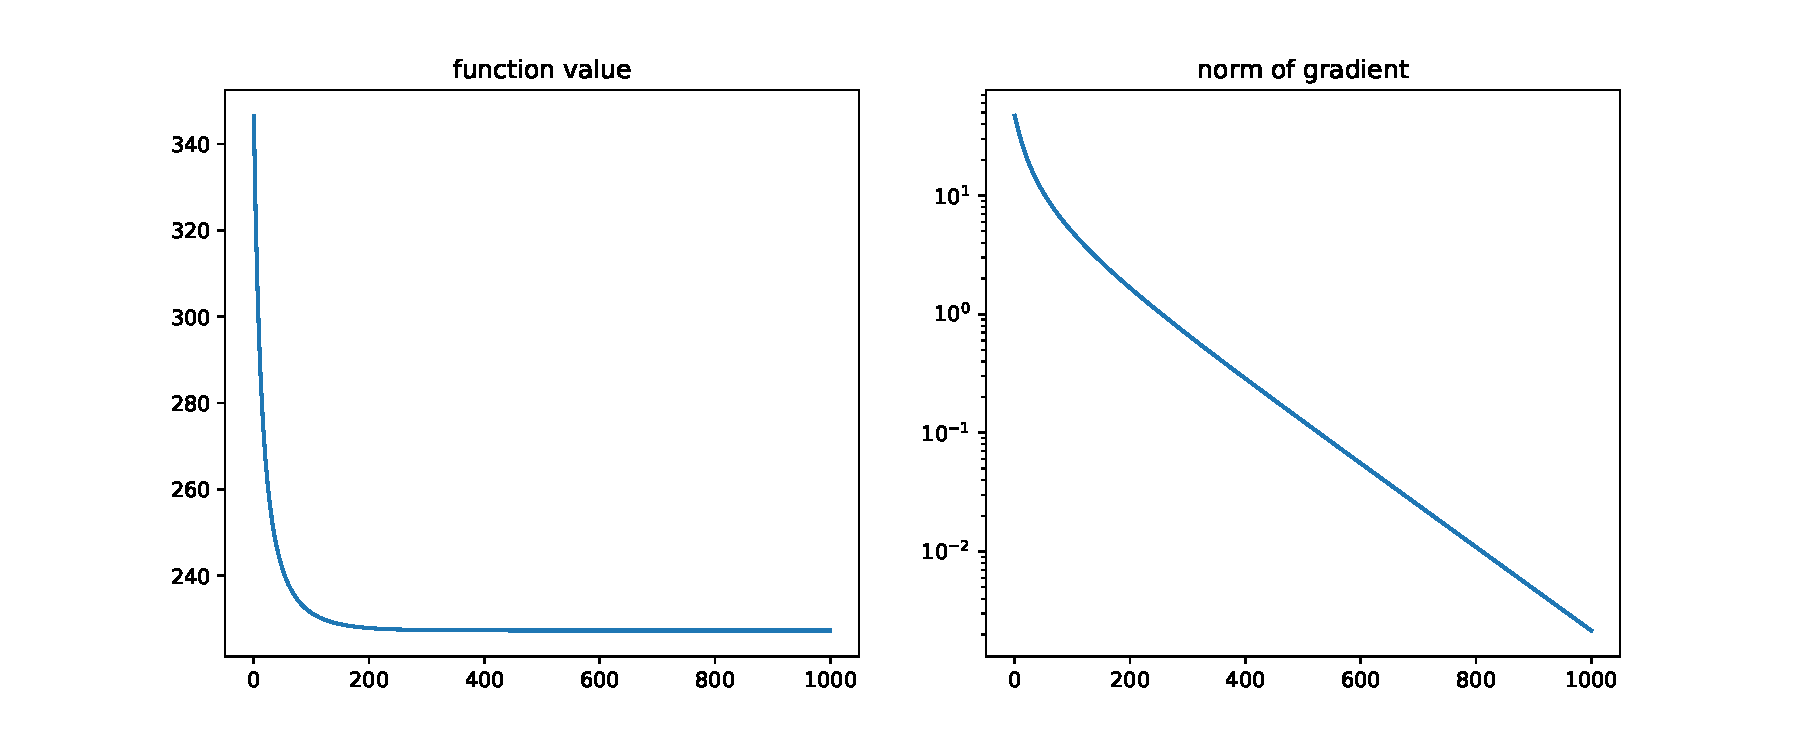
\includegraphics[width=0.7\textwidth]{img/logistic_gd.pdf}
            \caption{Gradient Descent on Logistic Regression}
            \label{logistic_gd}
        \end{figure}
        
    \item
        Figure~\ref{logistic_nm} shows the objective value (left) and norm of the gradient (right) vs iteration for Newton's method applied to \( \ell_2 \)-regularized logistic regression.
        \begin{figure}\centering
            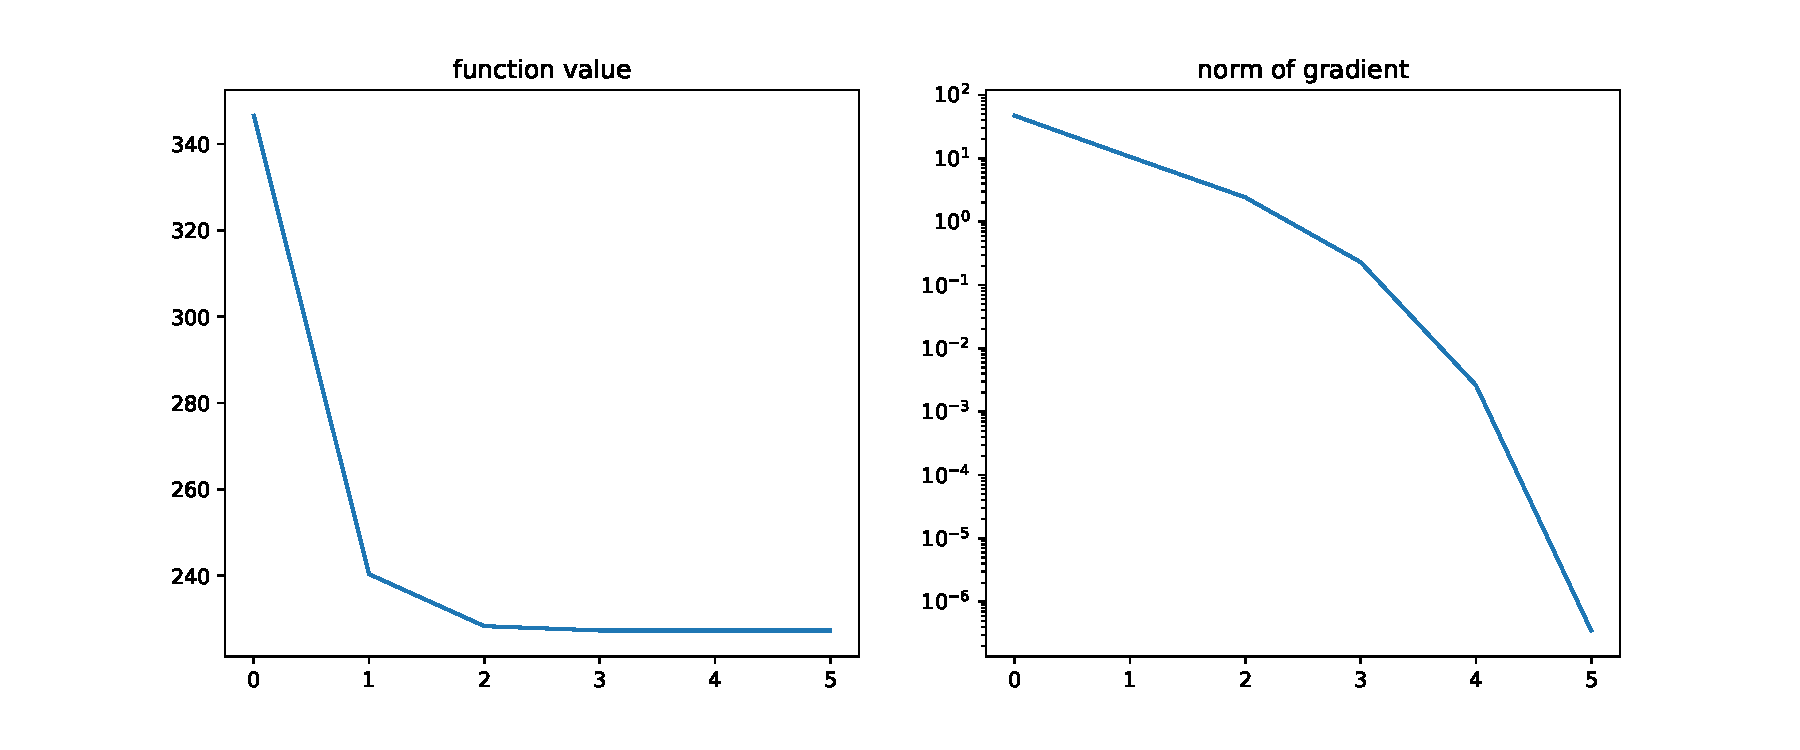
\includegraphics[width=0.7\textwidth]{img/logistic_nm.pdf}
            \caption{Newton's Method on Logistic Regression}
            \label{logistic_nm}
        \end{figure}
    \item
        Figures~\ref{poisson_gd} and \ref{poisson_nm} respectively show the objective value (left) and norm of the gradient (right) vs iteration for Gradient Descent and Newton's method applied to \( \ell_2 \)-regularized Poisson regression.
        \begin{figure}\centering
            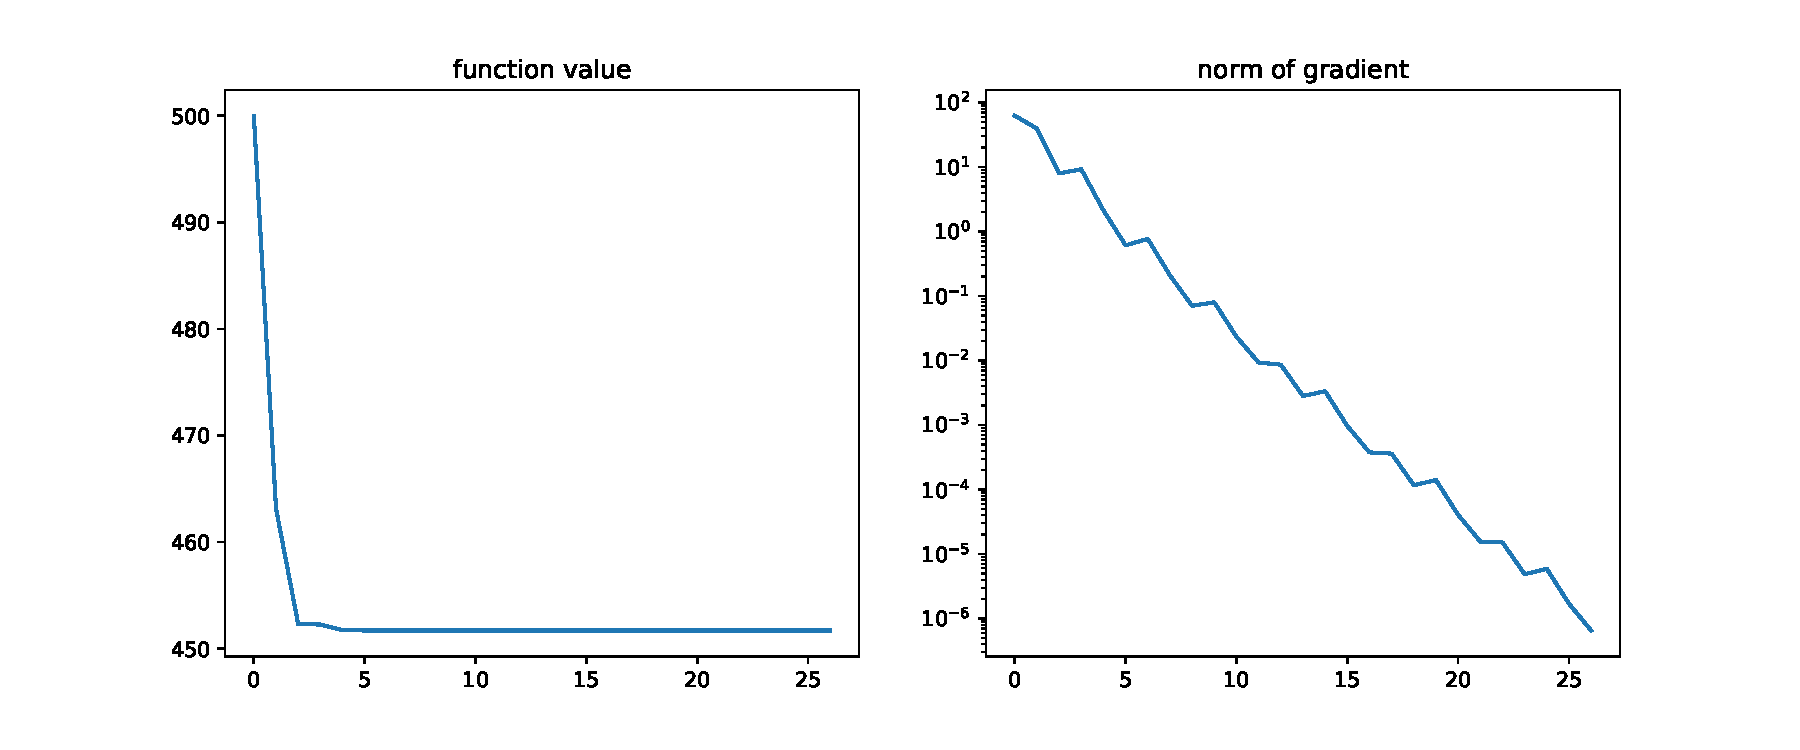
\includegraphics[width=0.7\textwidth]{img/poisson_gd.pdf}
            \caption{Gradient Descent on Poisson Regression}
            \label{poisson_gd}
        \end{figure}
        \begin{figure}\centering
            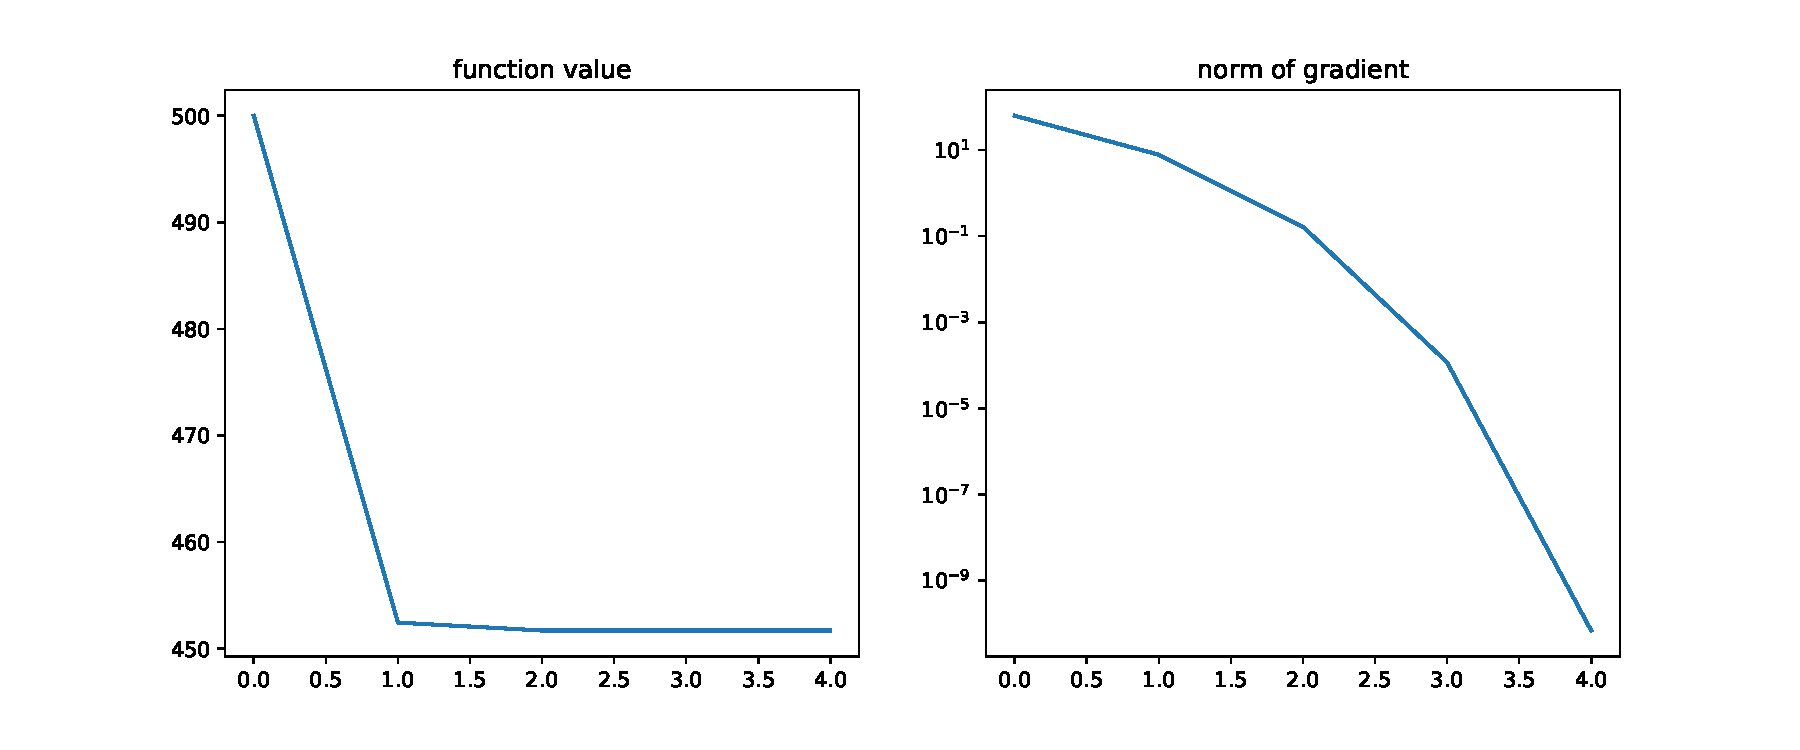
\includegraphics[width=0.7\textwidth]{img/poisson_nm.pdf}
            \caption{Newton's Method on Poisson Regression}
            \label{poisson_nm}
        \end{figure}
 

    \item The Newton solvers converge in many fewer steps. On the semilog plot of the gradient it is also clear that Newton's method begins to converge more quickly once the norm of the gradient is sufficiently small.

\end{enumerate}
\end{solution}

\clearpage
\begin{problem}[Bonus]
Consider the poisson model 
\[
P(b_i | \lambda_i) = \frac{1}{b_i!} \exp(-\lambda_i + b_i \ln(\lambda_i)).
\]

Develop an inference model for \( x \) by using the assumption \( \lambda_i = a_i^T x \). Write down an optimization problem, and 
solve it using a method of your choice. The \( \ln \) is only defined for positive inputs, so you want to make sure you start and 
stay feasible, i.e. that you never let \( x \) be such that any \( a_i^T x \) fall below \( 0 \).

Test your ability to predict outcomes  using  the standard Poisson model vs. your new model. 
One way to do this is to divide your dataset into `training' and `testing', solve for \( x \) using the training dataset, and evaluate how far you are
from the observed \( b_i \) on the test set. Include a table or plot that meaningfully compares the standard Poisson model vs. the one you developed here. 
Describe any implementation issues you encountered and what you learned. Do the patterns you observed hold over different realizations of sampled data? 
\end{problem}

\begin{solution}[Solution]
\end{solution}

\end{document}
